\begin{applicationActivities}

\begin{observation}
Let \(T: V \rightarrow W\).  We have previously defined the following
terms.
\begin{itemize}
\item  \(T\) is called \term{injective} or \term{one-to-one} if \(T\) does not map two distinct vectors to the same place.
\item \(T\) is called \term{surjective} or \term{onto} if every element of \(W\) is mapped to by some element of \(V\).
\item The \term{kernel} of \(T\) is the set of all vectors in \(V\) that are mapped to $\vec{z}\in W$.  It is a subspace of \(V\).
\item The \term{image} of \(T\) is the set of all vectors in \(W\) that are mapped to by something in \(V\).  It is a subspace of \(W\).
\end{itemize}
\end{observation}

\begin{activity}{5}
Let \(T: V \rightarrow W\) be a linear transformation where
\(\ker T\) contains multiple vectors. What can you conclude?
\begin{enumerate}[(a)]
\item \(T\) is injective
\item \(T\) is not injective
\item \(T\) is surjective
\item \(T\) is not surjective
\end{enumerate}
\end{activity}

\begin{fact}
A linear transformation $T$ is injective \textbf{if and only if} $\ker T = \{\vec{0}\}$. Put another way, an injective linear transformation may be
recognized by its \term{trivial} kernel.

\begin{center}
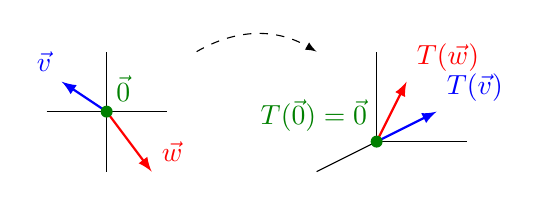
\begin{tikzpicture}[x=0.15in,y=0.15in]
  \begin{scope}[shift={(0,1)}]
    \draw (-2,0) -- (2,0);
    \draw (0,-2) -- (0,2);
    \draw[thick,-latex,blue] (0,0) -- (-1.5,1)
          node[anchor=south east] {\(\vec v\)};
    \draw[thick,-latex,red] (0,0) -- (1.5,-2)
          node[anchor=south west] {\(\vec w\)};
    \fill[green!50!black] (0,0) circle (0.2)
          node[anchor=south west] {\(\vec{0}\)};
  \end{scope}
  \draw[dashed,-latex] (3,3) to [bend left=30] (7,3);
  \begin{scope}[shift={(9,0)}]
    \draw (0,0) -- (3,0);
    \draw (0,0) -- (0,3);
    \draw (0,0) -- (-2,-1);
    \draw[thick,-latex,blue] (0,0) -- (2,1)
          node[anchor=south west] {\(T(\vec v)\)};
    \draw[thick,-latex,red] (0,0) -- (1,2)
          node[anchor=south west] {\(T(\vec w)\)};
    \fill[green!50!black] (0,0) circle (0.2)
          node[anchor=south east] {\(T(\vec{0})=\vec{0}\)};
  \end{scope}
\end{tikzpicture}
\end{center}
\end{fact}

\begin{activity}{5}
Let $T: \IR^5 \rightarrow \IR^5$ be a linear transformation where
$\Im T$ is spanned by four vectors.
What can you conclude?
\begin{enumerate}[(a)]
\item \(T\) is injective
\item \(T\) is not injective
\item \(T\) is surjective
\item \(T\) is not surjective
\end{enumerate}
\end{activity}

\begin{fact}
A linear transformation $T:V \rightarrow W$ is surjective \textbf{if and only if} $\Im T = W$. Put another way, a surjective linear transformation may be
recognized by its identical codomain and image.
\begin{center}
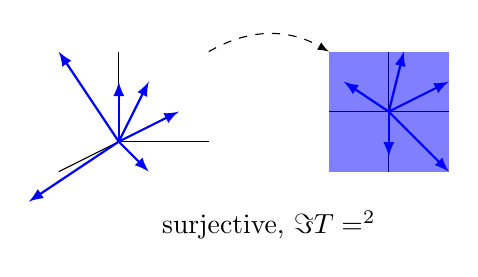
\begin{tikzpicture}[x=0.15in,y=0.15in]
  \begin{scope}[shift={(0,0)}]
    \draw (0,0) -- (3,0);
    \draw (0,0) -- (0,3);
    \draw (0,0) -- (-2,-1);
    \draw[thick,-latex,blue] (0,0) -- (2,1);
    \draw[thick,-latex,blue] (0,0) -- (1,2);
    \draw[thick,-latex,blue] (0,0) -- (0,2);
    \draw[thick,-latex,blue] (0,0) -- (1,-1);
    \draw[thick,-latex,blue] (0,0) -- (-2,3);
    \draw[thick,-latex,blue] (0,0) -- (-3,-2);
  \end{scope}
  \draw[dashed,-latex] (3,3) to [bend left=30] (7,3);
  \begin{scope}[shift={(9,1)}]
    \draw (-2,0) -- (2,0);
    \draw (0,-2) -- (0,2);
    \draw[thick,-latex,blue] (0,0) -- (0.5,2);
    \draw[thick,-latex,blue] (0,0) -- (2,1);
    \draw[thick,-latex,blue] (0,0) -- (-1.5,1);
    \draw[thick,-latex,blue] (0,0) -- (0,-1.5);
    \draw[thick,-latex,blue] (0,0) -- (2,-2);
    \fill[color=blue, opacity=0.5] (-2,-2) rectangle (2,2);
  \end{scope}
  \node[anchor=north] at (5,-2) {surjective, \(\Im T=\IR^2\)};
\end{tikzpicture}
\hspace{3em}
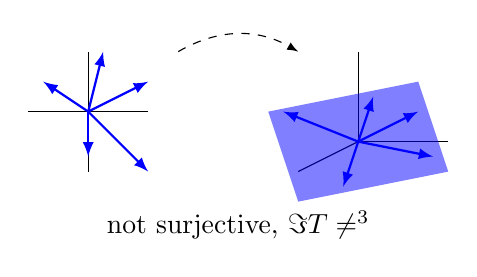
\begin{tikzpicture}[x=0.15in,y=0.15in]
  \begin{scope}[shift={(0,1)}]
    \draw (-2,0) -- (2,0);
    \draw (0,-2) -- (0,2);
    \draw[thick,-latex,blue] (0,0) -- (0.5,2);
    \draw[thick,-latex,blue] (0,0) -- (2,1);
    \draw[thick,-latex,blue] (0,0) -- (-1.5,1);
    \draw[thick,-latex,blue] (0,0) -- (0,-1.5);
    \draw[thick,-latex,blue] (0,0) -- (2,-2);
  \end{scope}
  \draw[dashed,-latex] (3,3) to [bend left=30] (7,3);
  \begin{scope}[shift={(9,0)}]
    \draw (0,0) -- (3,0);
    \draw (0,0) -- (0,3);
    \draw (0,0) -- (-2,-1);
    \draw[thick,-latex,blue] (0,0) -- (0.5,1.5);
    \draw[thick,-latex,blue] (0,0) -- (2,1);
    \draw[thick,-latex,blue] (0,0) -- (-2.5,1);
    \draw[thick,-latex,blue] (0,0) -- (-0.5,-1.5);
    \draw[thick,-latex,blue] (0,0) -- (2.5,-0.5);
    \fill[color=blue, opacity=0.5] (-2,-2) -- (3,-1) -- (2,2) -- (-3,1) -- (-2,-2);
  \end{scope}
  \node[anchor=north] at (5,-2) {not surjective, \(\Im T\not=\IR^3\)};
\end{tikzpicture}
\end{center}
\end{fact}

\begin{activity}{15}
Let $T: \IR^n \rightarrow \IR^m$ be a linear map with standard matrix $A$.
Sort the following claims into two groups of \textit{equivalent} statements:
one group that means \(T\) is \textbf{injective}, and one group that means
\(T\) is \textbf{surjective}.
\begin{multicols}{2}
\begin{enumerate}[(a)]
\item The kernel of \(T\) is trivial: \(\ker T=\{\vec 0\}\).
\item The columns of $A$ span $\IR^m$.
\item The columns of $A$ are linearly independent.
\item Every column of $\RREF(A)$ has a pivot.
\item Every row of $\RREF(A)$ has a pivot.
\item The image of \(T\) equals its codomain: \(\Im T=\IR^m\).
\item The system of linear equations given by the augmented matrix $\begin{bmatrix}[c|c]A & \vec{b} \end{bmatrix}$ has a solution for all $\vec{b} \in \IR^m$.
\item The system of linear equations given by the augmented matrix $\begin{bmatrix}[c|c] A & \vec{0} \end{bmatrix}$ has exactly one solution.
\end{enumerate}
\end{multicols}
\begin{instructorNote}
  This activity may be ran as a card sort.
\end{instructorNote}
\end{activity}

\begin{observation}
  The easiest way to show that the linear map with standard matrix \(A\)
  is injective is to show that \(\RREF(A)\) has all pivot columns.

  \vspace{1em}

  The easiest way to show that the linear map with standard matrix \(A\)
  is surjective is to show that \(\RREF(A)\) has all pivot rows.
\end{observation}

\begin{activity}{3}
  What can you immediately conclude about the linear map \(T:\IR^5\to\IR^3\)?
  \begin{enumerate}[a)]
    \item Its standard matrix has more columns than rows, so \(T\) is not
    \item Its standard matrix has more columns than rows, so \(T\) is 
    injective.
    \item Its standard matrix has more rows than columns, so \(T\) is not
    \item Its standard matrix has more rows than columns, so \(T\) is 
    surjective.
  \end{enumerate}
\end{activity}

\begin{activity}{2}
  What can you immediately conclude about the linear map \(T:\IR^2\to\IR^7\)?
  \begin{enumerate}[a)]
    \item Its standard matrix has more columns than rows, so \(T\) is not
    \item Its standard matrix has more columns than rows, so \(T\) is 
    injective.
    \item Its standard matrix has more rows than columns, so \(T\) is not
    \item Its standard matrix has more rows than columns, so \(T\) is 
    surjective.
  \end{enumerate}
\end{activity}

\begin{fact}
  The following are true for any linear map \(T:V\to W\):
  \begin{itemize}
    \item If \(\dim(V)>\dim(W)\), then \(T\) is not injective.
    \item If \(\dim(V)<\dim(W)\), then \(T\) is not surjective.
  \end{itemize}
  Basically, a linear transformation cannot reduce dimension without collapsing
  vectors into each other, and a linear transformation cannot
  increase the dimension of its image.
  \begin{multicols}{2}
  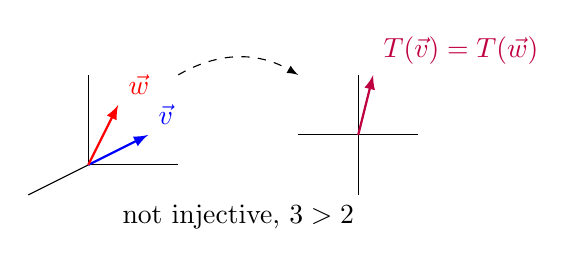
\begin{tikzpicture}[x=0.15in,y=0.15in]
    \begin{scope}[shift={(0,0)}]
      \draw (0,0) -- (3,0);
      \draw (0,0) -- (0,3);
      \draw (0,0) -- (-2,-1);
      \draw[thick,-latex,blue] (0,0) -- (2,1)
            node[anchor=south west] {\(\vec v\)};
      \draw[thick,-latex,red] (0,0) -- (1,2)
            node[anchor=south west] {\(\vec w\)};
    \end{scope}
    \draw[dashed,-latex] (3,3) to [bend left=30] (7,3);
    \begin{scope}[shift={(9,1)}]
      \draw (-2,0) -- (2,0);
      \draw (0,-2) -- (0,2);
      \draw[thick,-latex,purple] (0,0) -- (0.5,2)
            node[anchor=south west] {\(T(\vec v)=T(\vec w)\)};
    \end{scope}
    \node[anchor=north] at (5,-1) {not injective, \(3>2\)};
  \end{tikzpicture}

  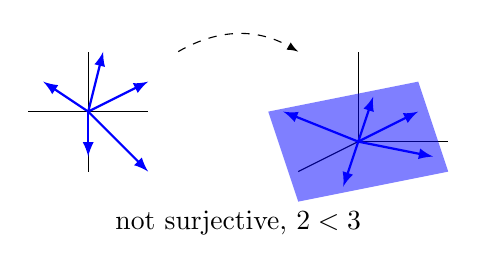
\begin{tikzpicture}[x=0.15in,y=0.15in]
    \begin{scope}[shift={(0,1)}]
      \draw (-2,0) -- (2,0);
      \draw (0,-2) -- (0,2);
      \draw[thick,-latex,blue] (0,0) -- (0.5,2);
      \draw[thick,-latex,blue] (0,0) -- (2,1);
      \draw[thick,-latex,blue] (0,0) -- (-1.5,1);
      \draw[thick,-latex,blue] (0,0) -- (0,-1.5);
      \draw[thick,-latex,blue] (0,0) -- (2,-2);
    \end{scope}
    \draw[dashed,-latex] (3,3) to [bend left=30] (7,3);
    \begin{scope}[shift={(9,0)}]
      \draw (0,0) -- (3,0);
      \draw (0,0) -- (0,3);
      \draw (0,0) -- (-2,-1);
      \draw[thick,-latex,blue] (0,0) -- (0.5,1.5);
      \draw[thick,-latex,blue] (0,0) -- (2,1);
      \draw[thick,-latex,blue] (0,0) -- (-2.5,1);
      \draw[thick,-latex,blue] (0,0) -- (-0.5,-1.5);
      \draw[thick,-latex,blue] (0,0) -- (2.5,-0.5);
      \fill[color=blue, opacity=0.5] (-2,-2) -- (3,-1) -- (2,2) -- (-3,1) -- (-2,-2);
    \end{scope}
    \node[anchor=north] at (5,-2) {not surjective, \(2<3\)};
  \end{tikzpicture}
  \end{multicols}
  But these results do \textbf{not} reverse. For example,
  \(T:\IR^5\to\IR^4\) might not be surjective, even though \(5\not<4\).
\end{fact}


\begin{definition}
If \(T: V \rightarrow W\) is both injective and surjective, it is called \term{bijective}.
\end{definition}

\begin{activity}{5}
Let $T: \IR^n \rightarrow \IR^m$ be a bijective linear map with
standard matrix $A$. Label each of the following as true or false.
\begin{enumerate}[(a)]
\item The columns of $A$ form a basis for $\IR^m$
\item $\RREF(A)$ is the identity matrix.
\item The system of linear equations given by the augmented matrix $\begin{bmatrix}[c|c] A & \vec{b} \end{bmatrix}$ has exactly one solution
for all \(\vect b \in \IR^m\).
\end{enumerate}
\end{activity}

\begin{observation}
  The easiest way to show that the linear map with standard matrix \(A\)
  is bijective is to show that \(\RREF(A)\) is the identity matrix.
\end{observation}

\begin{activity}{5}
Let $T: \IR^3 \rightarrow \IR^3$ be given by the standard matrix $$A=\begin{bmatrix} 2&1&-1 \\ 4&1&1 \\ 6&2&1\end{bmatrix}.$$ Which of the following must be true?
\begin{enumerate}[(a)]
\item $T$ is neither injective nor surjective
\item $T$ is injective but not surjective
\item $T$ is surjective but not injective
\item $T$ is bijective.
\end{enumerate}
\end{activity}

\begin{activity}{5}
Let $T: \IR^3 \rightarrow \IR^3$ be given by $$T\left(\begin{bmatrix} x \\ y  \\ z \end{bmatrix} \right) = \begin{bmatrix} 2x+y-z \\ 4x+y+z \\ 6x+2y\end{bmatrix}.$$   Which of the following must be true?
\begin{enumerate}[(a)]
\item $T$ is neither injective nor surjective
\item $T$ is injective but not surjective
\item $T$ is surjective but not injective
\item $T$ is bijective.
\end{enumerate}
\end{activity}


\end{applicationActivities}
